%!TEX root = Main.tex
\documentclass[Main]{subfiles}
\begin{document}

\section{Software} % (fold)
\label{sec:software}

	In this chapter, the coding environment, design and implementation of the software will be covered.
	For reference, the entire codebase can be found in \fxnote{CodeBae Reference}.
	
	\subsection{Environment} % (fold)
	\label{sub:software_environment}

		The software for this project was written in C++ using the Xilinx Software Development Kit.
		C++ was chosen because it is a object oriented language, which gives some clear advantages when working in a team.
		Furthermore, C++ has native support for an resizable array datatype known as a vector, which greatly reduced the complexity of manipulating arrays.
		The software was written for the C++11 standard, since this standard gave some advantages in initialisation of vectors.
		GitHub was used for version control	to manage and backup code.
		
	\subsection{Design} % (fold)
	\label{sub:software_design}

	\subsubsection{Structure} % (fold)
	\label{subsub:software_structure}
		A object-oriented approach was taken to the design, in order to modulize the different parts of the software. 
		
		This gave clear advantages when working multiple people on the same codebase, as the development of the different classes could be spread out between multiple people.
		
		The structure of the software is depicted in \autoref{fig:classdiagram} as a UML class diagram.
		
		The main components of the program is the LIDAR, PathMaker, RobotFrame and ParticleFilter classes. 
		Each class has a distinct purpose, which maps directly to one of the four  actions in the main loop of \autoref{fig:systemact}.
		The mapping can be see in \autoref{table:action_class_map}
		 
		\begin{table}[H]
			\centering
			\begin{tabular}{|c|c|}
			\hline
				Action & Class \\ 
			\hline
				A2: Sense Data & LIDAR  \\ 
			\hline
				A3: Estimate Robot Position & ParticleFilter  \\ 
			\hline
				A4: Calculate Path & PathMaker  \\ 
			\hline
				A5: Move & RobotFrame  \\ 
			\hline
			\end{tabular}
			\caption{Action mapping of classes}
			\label{table:action_class_map} 
		\end{table} \noindent
		
		\begin{figure}[H]
			\centering
			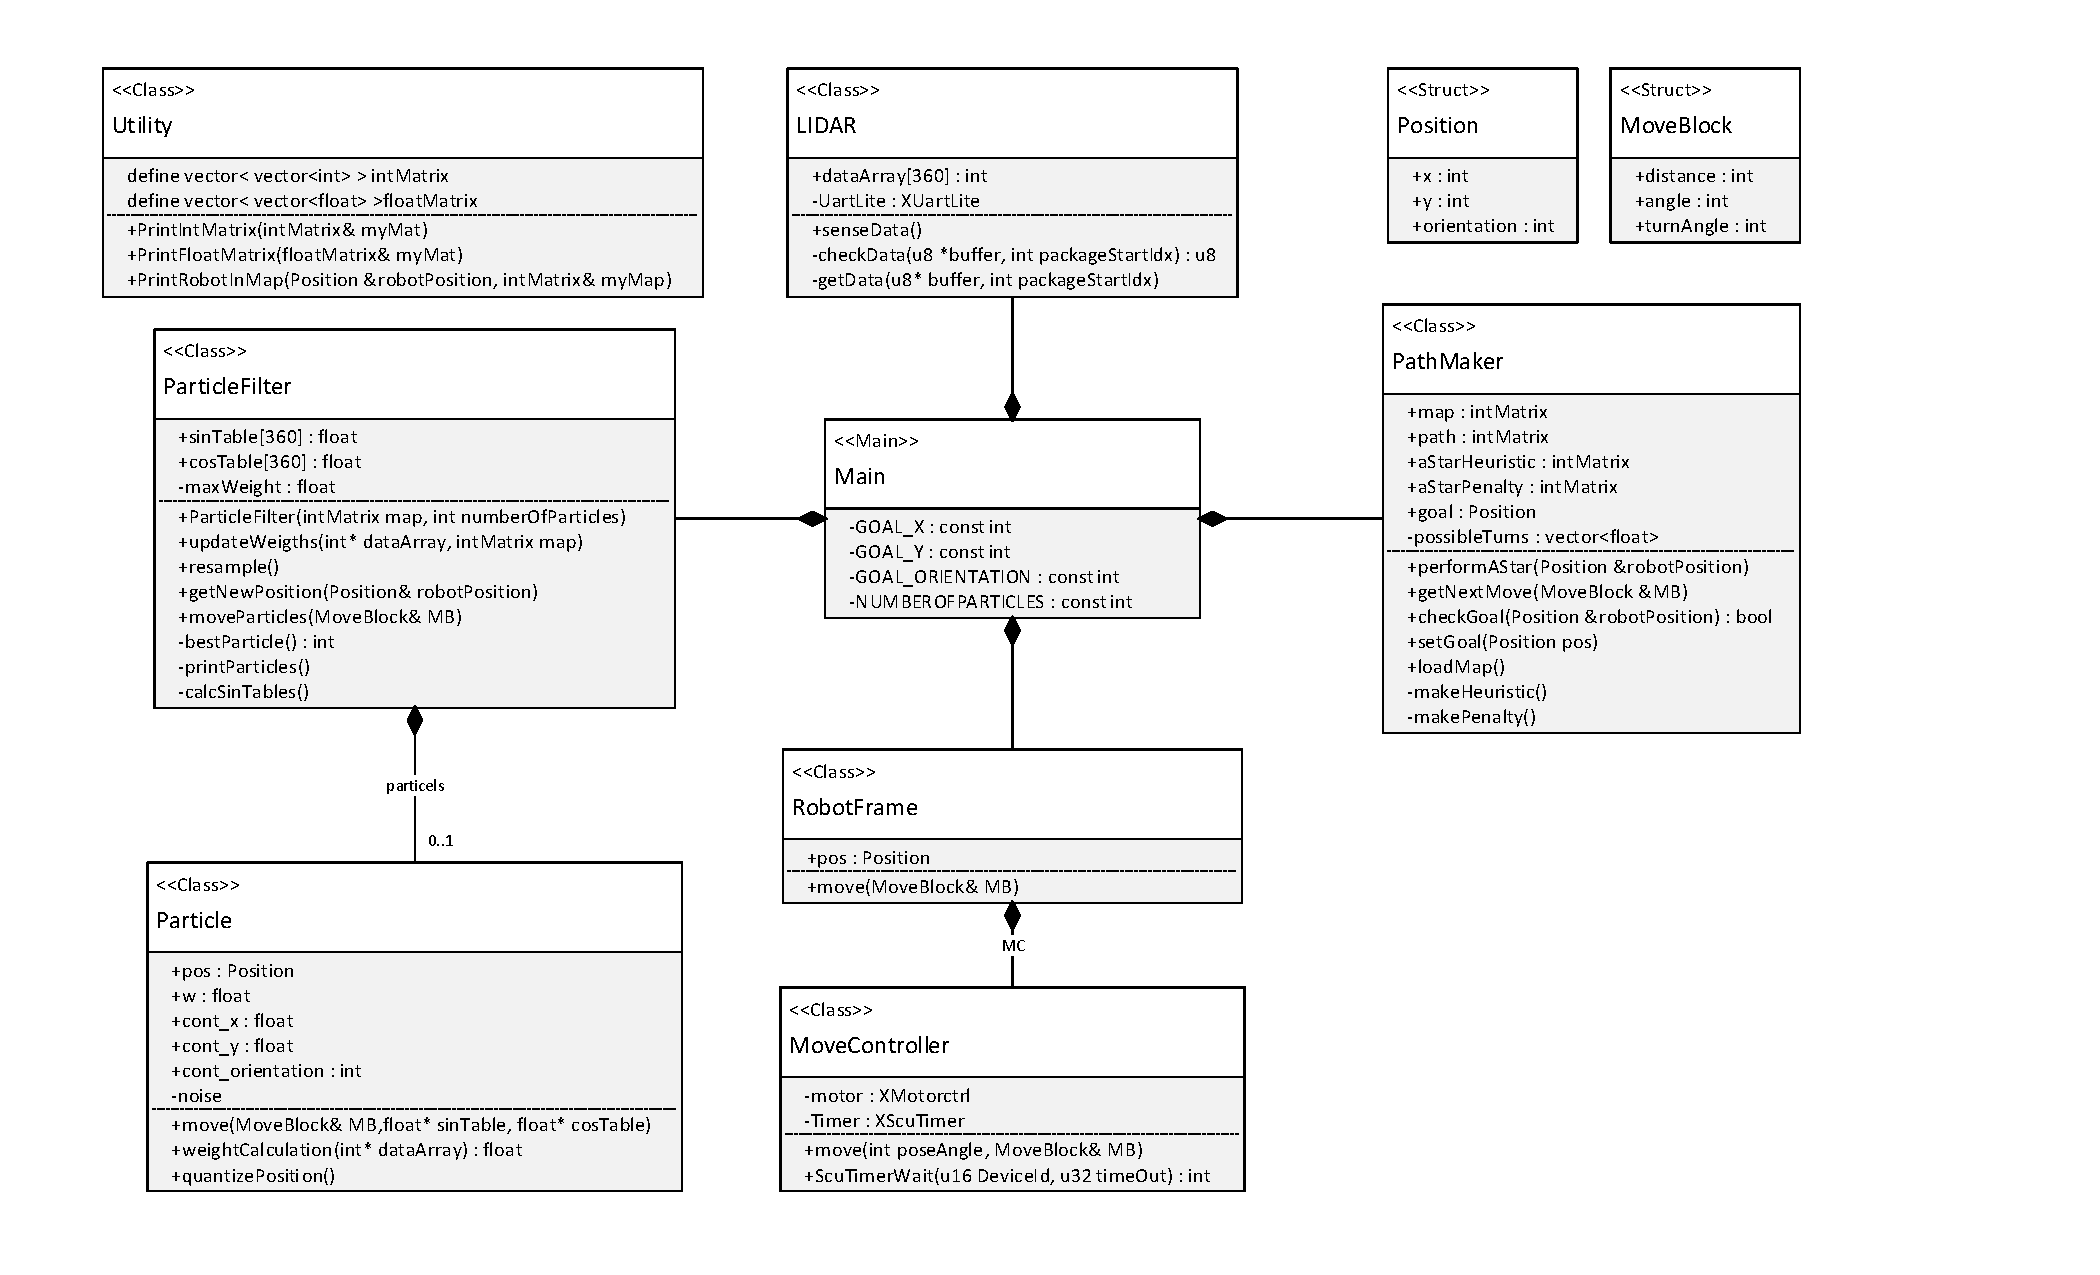
\includegraphics[width=\linewidth]{ClassDiagram}
			\caption{Class Diagram}
			\label{fig:classdiagram}
		\end{figure}
		
	\subsubsection{Behaviour} % (fold)
	\label{subsub:software_behaviour}

		The dataflow between the different classes is covered in the Internal Block Diagram in \autoref{fig:softwareibd}.

		The raw sensor data from the Sensing block in \autoref{fig:systemibd} is sent to the LIDAR class, which  converts the raw sensor data to 360 distance values.
		The sensor data is sent to the ParticleFilter class, which updates its current particle weights. 
		These weights are used to resample the particles using the Low Variance Resampling technique presented in the course material, \autoref{sec:particlefilter}.
		The robots position is then estimated as position and orientation of the particle with the largest weight.
		This position is used in the PathMaker, which performs AStar to find the best path to the goal. 

		The next move from this path is sent to both the RobotFrame class and the ParticleFilter, to move both the robot and the particles along the expected path.
		The RobotFrame class uses the MotorControl class to send a control signal to the Motion block from \autoref{fig:systemibd}, which converts the control to a PWM signal that controls the motors of the robot.
		
		
		\begin{figure}[H]
			\centering
			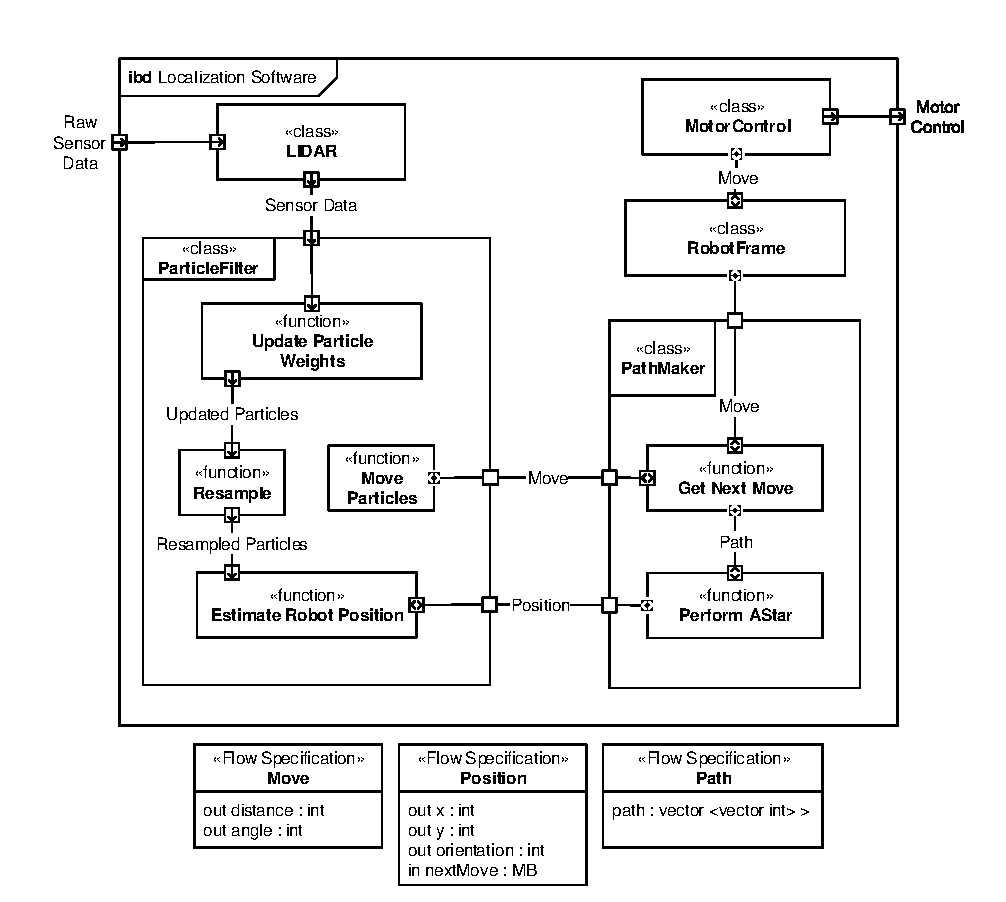
\includegraphics{SoftwareIBD}
			\caption{Software Internal Block Diagram}
			\label{fig:softwareibd}
		\end{figure}
	
	\subsection{Implementation} % (fold)
	\label{sub:software_implementation}
	
	This section covers the implementation specific details of the software.
	The software was implemented according to the design, as the programs main function, presented in \autoref{lst:main_code}, makes apparent.

	Focus in the following subsections has been put on the PathMaker, ParticleFilter and RobotFrame class, as they have required the most work during implementation.

	\newpage
	\begin{lstlisting}[caption=Main Function of Progam, style=Code-C++, label=lst:main_code, basicstyle=\scriptsize]
	int main(void) {
		Position goal;
		goal.x = GOAL_X;
		goal.y = GOAL_Y;
		goal.orientation = GOAL_ORIENTATION;
	
		PathMaker* pathMaker = new PathMaker();
		pathMaker->setGoal(goal);
		pathMaker->loadMap();
	
		RobotFrame* robotFrame = new RobotFrame();
		robotFrame->pos.x = 4;
		robotFrame->pos.y = 4;
	
		ParticleFilter* particleFilter = new ParticleFilter(pathMaker->map);
		LIDAR* lidar = new LIDAR();
		MoveBlock nextMove;
	
		while (1) {
			if (pathMaker->checkGoal(robotFrame->pos) != true) {
				
				lidar->senseData();
				
				particleFilter->updateWeigths(lidar->dataArray, pathMaker->map);
				particleFilter->resample(pathMaker->map);
				particleFilter->getNewPosition(robotFrame->pos);
				
				pathMaker->performAStar(robotFrame->pos);
				pathMaker->getNextMove(nextMove);
				
				robotFrame->move(nextMove);
				particleFilter->moveParticles(nextMove);
			}
			else
			{
				std::cout << "Found Goal" << std::endl;
				return 0;
			}
		}
		return 0;
	}
	
	\end{lstlisting}
	
	\subsubsection{ParticleFilter} % (fold)
	\label{subsub:software_particlefilter}
	
	The ParticleFilter class is responsible for turning  sensor data into an estimate of the robots current position. 
	In this course, the two main techniques for doing so are particle filters and Kalman filters. 
	Particle filters were chosen, which the name of this class implies, since particle filters are relatively easy to implement, and do not require landmarks; it can use raw measurements.
	
	The ParticleFilter class uses a Particle object to represent a particle. A particle has attributes describing its position and orientation, much like the robot does. 
	These particles are generated randomly in the constructor of the ParticleFilter class.
	The ParticleFilter class has three main functions.
	UpdateWeights, Resample and GetNewPosition.
	The UpdateWeights function updates the weights of the particles. 
	The weights are calculated by using the weightCalculation function of the particle objects that can be seen in \autoref{lst:weightCalculation}.
	
	\begin{lstlisting}[caption=weightCalculation function of particle class, style=Code-C++, label=lst:weightCalculation, basicstyle=\scriptsize]
			
		float Particle::weightCalculation(int* dataArray){
	    
	    float prob = 0.0;
	    int distDif, angleIndex;
	    int measurement[NUM_ANGLES]; //[8];
	
	    for (int i = 0; i < NUM_ANGLES ; i++ ) {
	    	measurement[i] = dataArray[2*i];
	    }
	
	    int n = 0;
	    for(int i = 0; i < NUM_ANGLES; i++){
	        if (measurement[i] != -1){
	        
	        	angleIndex = modu(((pos.orientation/2)+i),180);
	            
	            distDif = RangeArray[pos.y][pos.x][angleIndex] - measurement[i];
	            prob += (normalizer - 0.5*(pow(distDif,2))/(noiseSqr));
	            n++;
	        }
	    }
	    
	    if(n == 0)
	        return 0;
	    else
	        return exp(prob/(float)n);
		}

	\end{lstlisting}
	
	The measured data is compared with the RangeArray. The RangeArray is a pre-computed array with 32x32x180 floats, that contains the expected measurement data at all grid cells and angels in the map.
		
	As described in \autoref{sec:particlefilter} the weight can be calculated using a Gaussian distribution.
	Since each particle compares 180 measurements with their expected ranges, the weights must be calculated as the product of likelihoods, that are found using a Gaussian.
	There is however a disadvantage using the likelihood directly due to that fact that it in numeric unstable because small numbers might be multiplied together.
	It is instead preferable to use the log likelihood while it turns the multiplications into additions, and then in the end find the likelihood by taking the exponential to the log likelihood value.
	In this project the log likelihood is being divided by the number of measurement used in the iteration before it is turned into likelihood.
	Thereby the weight is found as the likelihood given the exponential of the average log likelihood, \autoref{eq:weight_calc}	
	\begin{equation}
	\label{eq:weight_calc}
	w_i = \mathcal{L} (\mathbf{x}_i|\mathbf{z}) = \exp \left( \frac{1}{N} \displaystyle\sum_k \ln \left( \frac{1}{\sqrt{2\pi^2 \cdot \sigma_\mathbf{z}^2}} \exp \left( - \frac{\frac{1}{2}\cdot (z_k-x_{i,k})^2}{\sigma_\mathbf{z}^2} \right) \right) \right)
	\end{equation}
	
	\newpage
	Once the new weights have been calculated, the Resampling function is invoked. 
	The resampling function is the heart of the particle filter.
	In this function, a new set of particles is constructed, by randomly choosing particles from the current set.
	When choosing which particles to include in the new set, the probability of picking a certain particle is proportional to its weight.
	This is accomplished by using the Low Variance Resampling technique presented in the course material.

	Only 95$\%$ of the particles in the new set are made from resampling.
	The last 5$\%$ are new particles, which are randomly placed on the map.
	The randomly placed particles are needed if the robot misplaces itself in relations to its particle.
	This can happen if the movement of the robot does not fit the motion model, or if the robot is physically moved by someone else or "Kidnapped"; hence the "kidnapped robot" situation described in \autoref{sec:particlefilter}. 
	The Resampling function can be seen in \autoref{lst:resample}
	\vspace{12pt}
	\begin{lstlisting}[caption=Resampling function of ParticleFilter, style=Code-C++, label=lst:resample, basicstyle=\scriptsize]
		void ParticleFilter::resample(intMatrix map) {
			vector<Particle> tempSet;
			int index = rand() % NUMBEROFPARTICLES;
			float beta = 0;
			float r;
		
			//Resampling of old particles
			for (int i = 0; i < NUMBEROFPARTICLES-NUMBEROFRANDOMPARTICLES; i++) {
				r = static_cast<float>(rand()) / static_cast<float>(RAND_MAX);
				beta += r * 2 * maxWeight;
				while (beta > particles[index].w) {
					beta -= particles[index].w;
					index = (index + 1) % NUMBEROFPARTICLES;
				}
				tempSet.push_back(particles[index]);
			}
		
			//Newly generated random particels
			Particle tempPar;
			for(int i = 0; i < NUMBEROFRANDOMPARTICLES; i++){
		
				tempPar.cont_x = (static_cast <float> (rand()) / static_cast <float> (RAND_MAX/MAPWIDTH))*GRID_SIZE;
				tempPar.cont_y = (static_cast <float> (rand()) / static_cast <float> (RAND_MAX/MAPHEIGHT))*GRID_SIZE;
	
				tempPar.pos.x = (int)(tempPar.cont_x/GRID_SIZE);
				tempPar.pos.y = (int)(tempPar.cont_y/GRID_SIZE);
		
				if(map[tempPar.pos.y][tempPar.pos.x] == 0)
				{
					tempPar.cont_orientation = (rand()%4)*90; // Initialize particles in grid orientations
					tempPar.w = 0;
					tempSet.push_back(tempPar);
				}
				else
				{
					--i;
				}
			}
			particles = tempSet;
	
		}	
	\end{lstlisting}

	Lastly the particle filter estimates the most probable current position of the robot. 
	This is done by finding the particle with the largest weight.
	The course material proposes to do this by averaging the parameters of all particles.
	However, this does not work well with a multi-model distribution of particles.
	If the particles are clustered in two equally likely clusters, the resulting position would always be in between the two clusters, and thus wrong.
	By using the largest weight, the position would only be wrong half the time.
	
	Once the PathMaker class has used the estimate of the current position to find the next movement instructions for the robot, the same instructions are sent to the ParticleFilter.
	The movement instructions are applied to all the particles, with a normal distributed noise with standard deviation of 10$\degree$ added to the angle, and a normal distributed noise with standard deviation of 10 mm added to the distance.
	
		\subsubsection{PathMaker} % (fold)
	\label{subsub:software_pathmaker}
	
	The PathMaker class is responsibly for managing the map the robot is navigating in, finding the shortest path to the goal position and getting the next move instruction that moves the robot and the particles along the generated path.
	In the constructor of the PathMaker, a 32 x 32 grid is build, based on the real environment, shown in \autoref{fig:real_world}. 
	\vspace{12pt} 
	\begin{figure}[H]
		\centering
		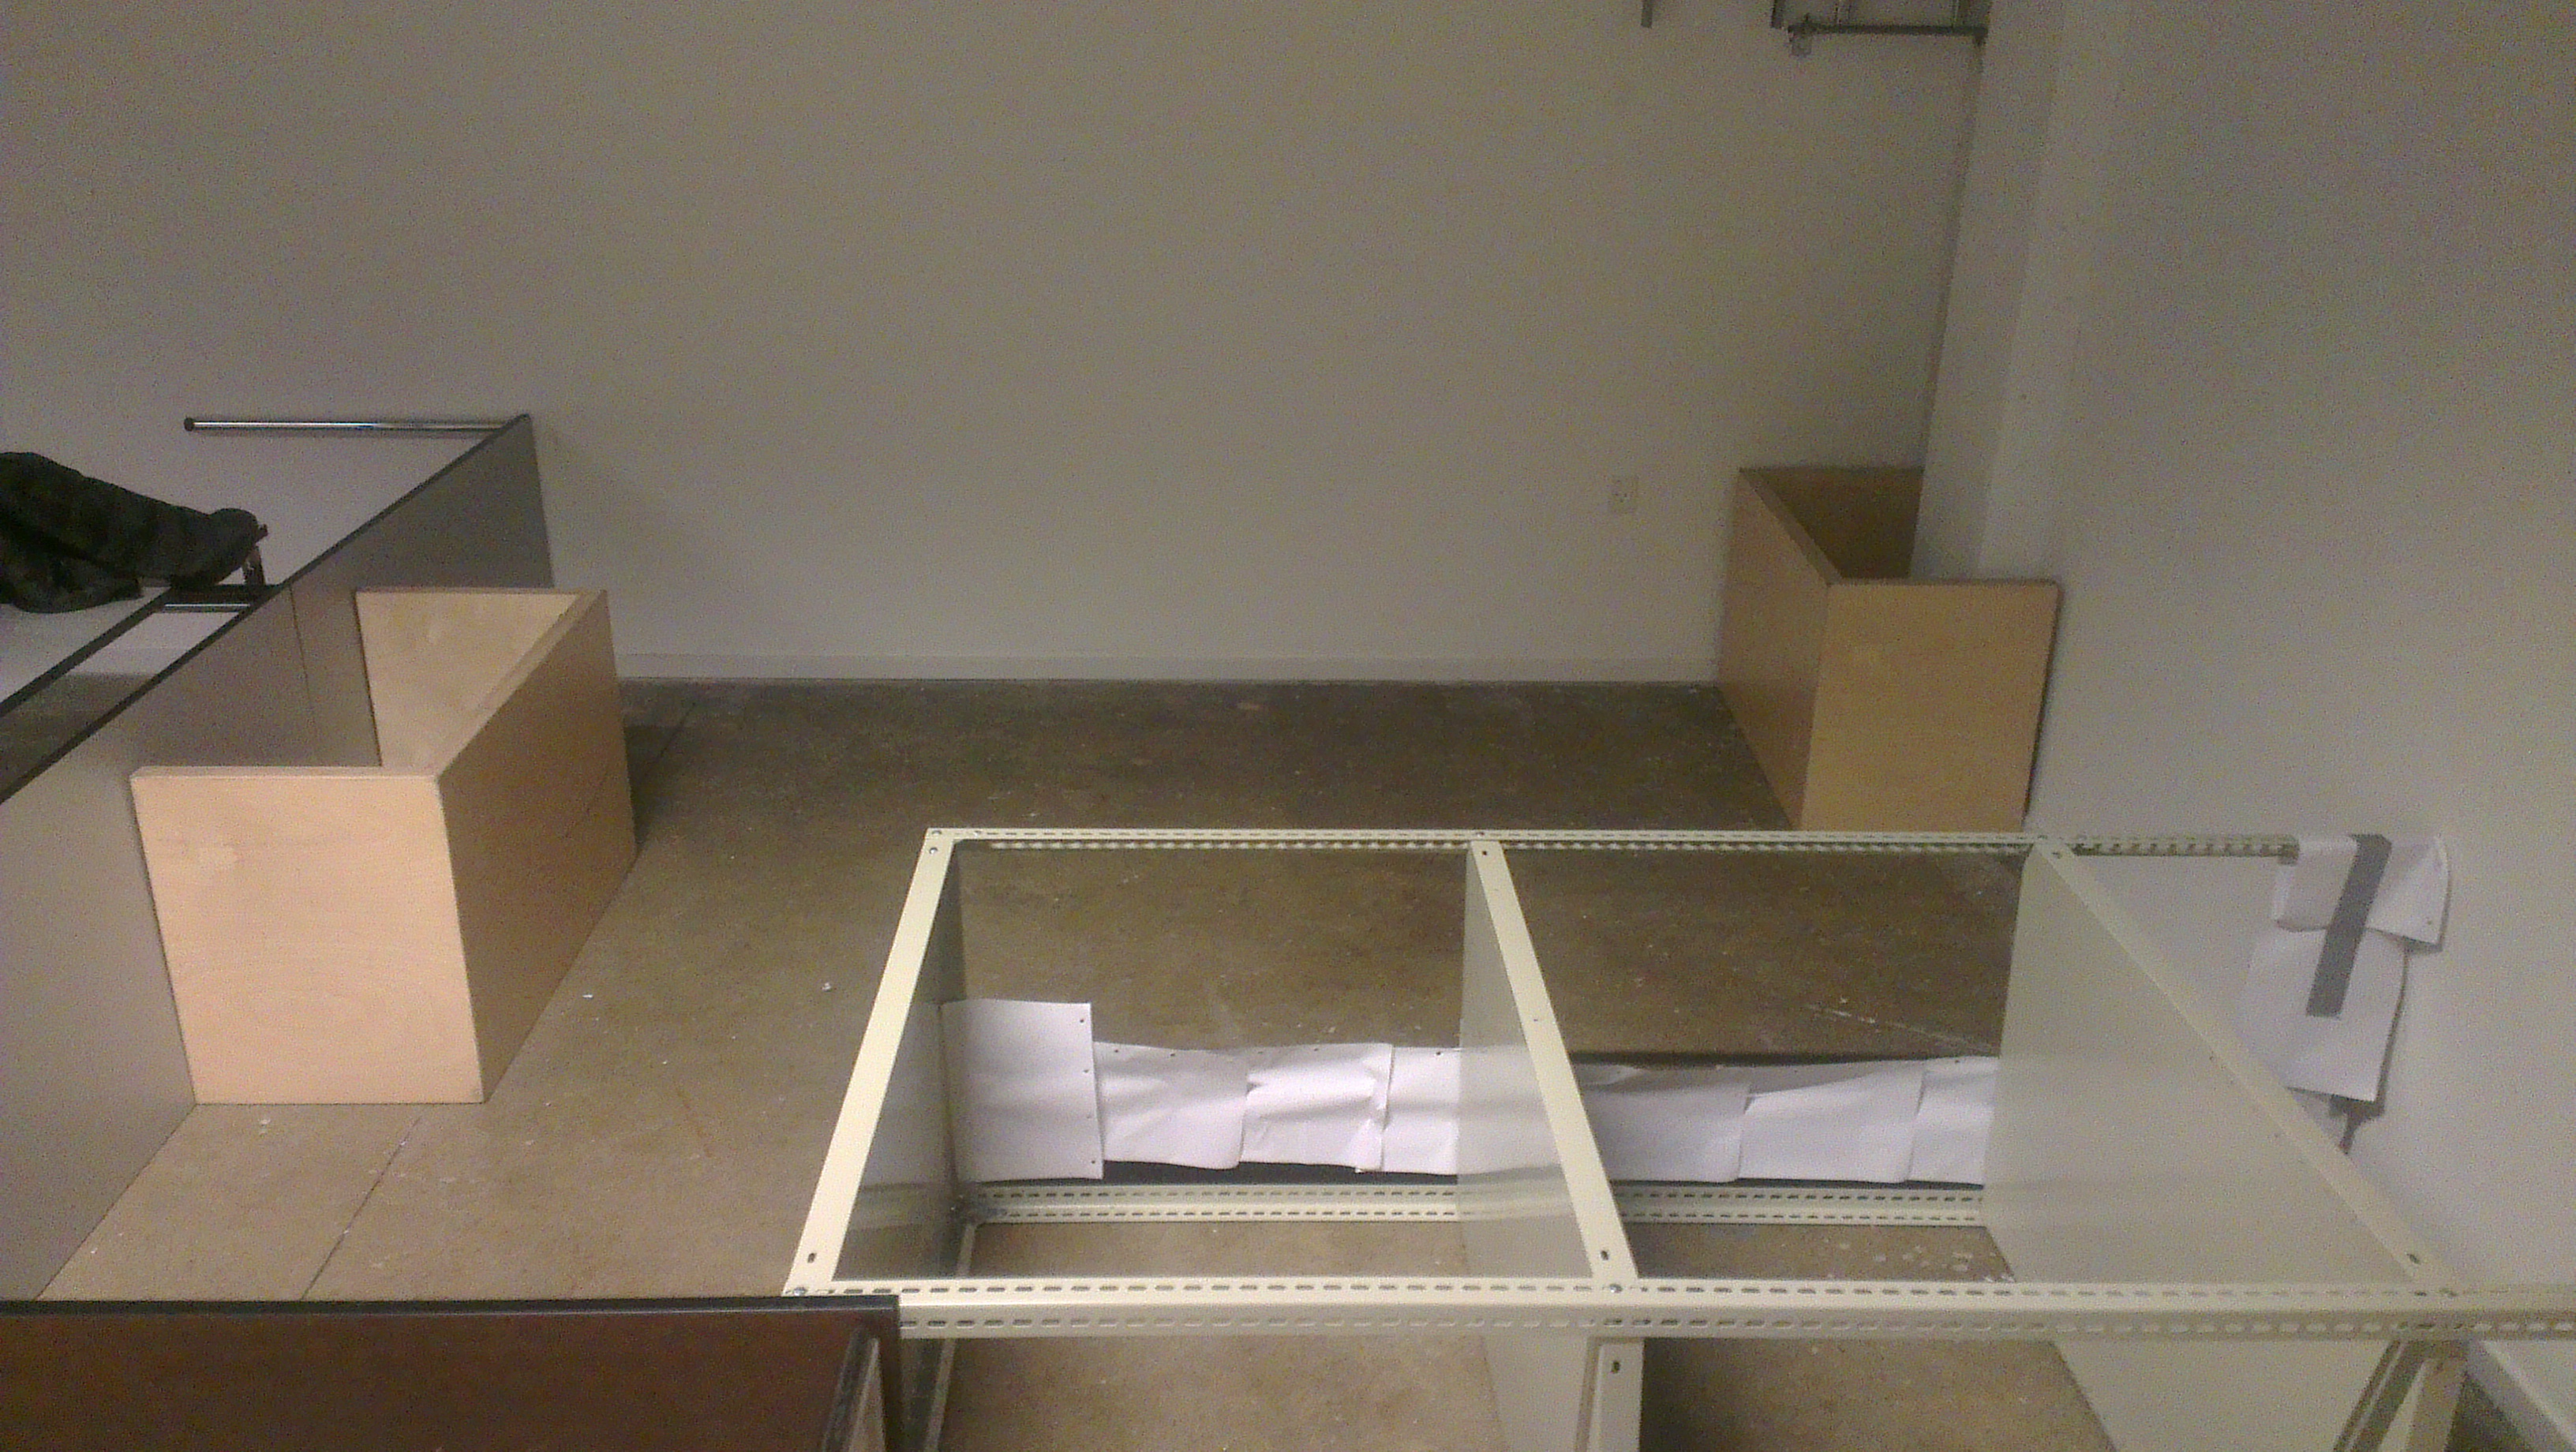
\includegraphics[width=1.0\linewidth]{CourseImage}
		\caption{Real-world environment}
		\label{fig:real_world}
	\end{figure}

	\newpage
	The grid map in which the robot will be driving, is divided into 10 x 10 cm squares. 
	Open spaces are represented as '0', Obstacles are represented as '1' and the robot is represented as '**'. The grid map can be seen in \autoref{table:realmap}.	

	\begin{table}[H]
		\centering
		\resizebox{\textwidth}{!}{
			\begin{tabular}{cccccccccccccccccccccccccccccccccc}
			\textbf{idx} & \textbf{ 0} & \textbf{ 1} & \textbf{ 2} & \textbf{ 3} & \textbf{ 4} & \textbf{ 5} & \textbf{ 6} & \textbf{ 7} & \textbf{ 8} & \textbf{ 9} & \textbf{10} & \textbf{11} & \textbf{12} & \textbf{13} & \textbf{14} & \textbf{15} & \textbf{16} & \textbf{17} & \textbf{18} & \textbf{19} & \textbf{20} & \textbf{21} & \textbf{22} & \textbf{23} & \textbf{24} & \textbf{25} & \textbf{26} & \textbf{27} & \textbf{28} & \textbf{29} & \textbf{30} & \textbf{31} \\
			\textbf{ 0} &  0 &  0 &  0 &  0 &  0 &  0 &  0 &  0 &  0 &  0 &  0 &  0 &  0 &  0 &  0 &  0 &  0 &  0 &  0 &  0 &  0 &  0 &  0 &  0 &  0 &  0 &  0 &  1 &  1 &  1 &  1 &  1 \\
			\textbf{ 1} &  0 &  0 &  0 &  0 &  0 &  0 &  0 &  0 &  0 &  0 &  0 &  0 &  0 &  0 &  0 &  0 &  0 &  0 &  0 &  0 &  0 &  0 &  0 &  0 &  0 &  0 &  0 &  1 &  1 &  1 &  1 &  1 \\
			\textbf{ 2} &  0 &  0 &  0 &  0 &  0 &  0 &  0 &  0 &  0 &  0 &  0 &  0 &  0 &  0 &  0 &  0 &  0 &  0 &  0 &  0 &  0 &  0 &  0 &  0 &  0 &  0 &  0 &  1 &  1 &  1 &  1 &  1 \\
			\textbf{ 3} &  0 &  0 &  0 &  0 &  0 &  0 &  0 &  0 &  0 &  0 &  0 &  0 &  0 &  0 &  0 &  0 &  0 &  0 &  0 &  0 &  0 &  0 &  0 &  0 &  0 &  0 &  0 &  1 &  1 &  1 &  1 &  1 \\
			\textbf{ 4} &  0 &  0 &  0 &  0 &  0 &  0 &  0 &  0 &  0 &  0 & ** &  0 &  0 &  0 &  0 &  0 &  0 &  0 &  0 &  0 &  0 &  0 &  0 &  0 &  0 &  0 &  0 &  1 &  1 &  1 &  1 &  1 \\
			\textbf{ 5} &  0 &  0 &  0 &  0 &  0 &  0 &  0 &  0 &  0 &  0 &  0 &  0 &  0 &  0 &  0 &  0 &  0 &  0 &  0 &  0 &  0 &  0 &  0 &  0 &  0 &  0 &  0 &  1 &  1 &  1 &  1 &  1 \\
			\textbf{ 6} &  0 &  0 &  0 &  0 &  0 &  0 &  0 &  0 &  0 &  0 &  0 &  0 &  0 &  0 &  0 &  0 &  0 &  0 &  0 &  0 &  0 &  0 &  0 &  0 &  0 &  0 &  0 &  1 &  1 &  1 &  1 &  1 \\
			\textbf{ 7} &  0 &  0 &  0 &  0 &  0 &  0 &  0 &  0 &  0 &  0 &  0 &  0 &  0 &  0 &  0 &  0 &  0 &  0 &  0 &  0 &  0 &  0 &  0 &  0 &  0 &  0 &  0 &  1 &  1 &  1 &  1 &  1 \\
			\textbf{ 8} &  0 &  0 &  0 &  0 &  0 &  0 &  0 &  0 &  0 &  0 &  0 &  0 &  0 &  0 &  0 &  0 &  0 &  0 &  0 &  0 &  0 &  0 &  0 &  0 &  0 &  0 &  0 &  1 &  1 &  1 &  1 &  1 \\
			\textbf{ 9} &  0 &  0 &  0 &  0 &  0 &  0 &  0 &  0 &  0 &  0 &  0 &  0 &  0 &  0 &  0 &  0 &  0 &  0 &  0 &  0 &  0 &  0 &  0 &  0 &  0 &  0 &  0 &  1 &  1 &  1 &  1 &  1 \\
			\textbf{10} &  1 &  1 &  1 &  1 &  1 &  0 &  0 &  0 &  0 &  0 &  0 &  0 &  0 &  0 &  0 &  0 &  0 &  0 &  0 &  0 &  0 &  0 &  0 &  0 &  0 &  0 &  0 &  0 &  0 &  0 &  0 &  0 \\
			\textbf{11} &  1 &  1 &  1 &  1 &  1 &  0 &  0 &  0 &  0 &  0 &  0 &  0 &  0 &  0 &  0 &  0 &  0 &  0 &  0 &  0 &  0 &  0 &  0 &  0 &  0 &  0 &  0 &  0 &  0 &  0 &  0 &  0 \\
			\textbf{12} &  1 &  1 &  1 &  1 &  1 &  0 &  0 &  0 &  0 &  0 &  0 &  0 &  0 &  0 &  0 &  0 &  0 &  0 &  0 &  0 &  0 &  0 &  0 &  0 &  0 &  0 &  0 &  0 &  0 &  0 &  0 &  0 \\
			\textbf{13} &  1 &  1 &  1 &  1 &  1 &  0 &  0 &  0 &  0 &  0 &  0 &  0 &  0 &  0 &  0 &  0 &  0 &  0 &  0 &  0 &  0 &  0 &  0 &  0 &  0 &  0 &  0 &  0 &  0 &  0 &  0 &  0 \\
			\textbf{14} &  1 &  1 &  1 &  1 &  1 &  0 &  0 &  0 &  0 &  0 &  0 &  0 &  0 &  0 &  0 &  0 &  0 &  0 &  0 &  0 &  0 &  0 &  0 &  0 &  0 &  0 &  0 &  0 &  0 &  0 &  0 &  0 \\
			\textbf{15} &  1 &  1 &  1 &  1 &  1 &  0 &  0 &  0 &  0 &  0 &  0 &  0 &  0 &  0 &  0 &  0 &  0 &  0 &  0 &  0 &  0 &  0 &  0 &  0 &  0 &  0 &  0 &  0 &  0 &  0 &  0 &  0 \\
			\textbf{16} &  1 &  1 &  1 &  1 &  1 &  0 &  0 &  0 &  0 &  0 &  0 &  0 &  0 &  0 &  0 &  0 &  0 &  0 &  0 &  0 &  0 &  0 &  0 &  0 &  0 &  0 &  0 &  0 &  0 &  0 &  0 &  0 \\
			\textbf{17} &  1 &  1 &  1 &  1 &  1 &  0 &  0 &  0 &  0 &  0 &  0 &  0 &  0 &  0 &  0 &  0 &  0 &  0 &  0 &  0 &  0 &  0 &  0 &  0 &  0 &  0 &  0 &  0 &  0 &  0 &  0 &  0 \\
			\textbf{18} &  1 &  1 &  1 &  1 &  1 &  0 &  0 &  0 &  0 &  0 &  0 &  0 &  0 &  0 &  0 &  0 &  0 &  0 &  0 &  0 &  0 &  0 &  0 &  0 &  0 &  0 &  0 &  0 &  0 &  0 &  0 &  0 \\
			\textbf{19} &  0 &  0 &  0 &  0 &  0 &  0 &  0 &  0 &  0 &  0 &  0 &  0 &  0 &  0 &  0 &  0 &  0 &  0 &  0 &  0 &  0 &  0 &  0 &  0 &  0 &  0 &  0 &  0 &  0 &  0 &  0 &  0 \\
			\textbf{20} &  0 &  0 &  0 &  0 &  0 &  0 &  0 &  0 &  0 &  0 &  0 &  0 &  0 &  0 &  0 &  0 &  0 &  0 &  0 &  0 &  0 &  0 &  0 &  0 &  0 &  0 &  0 &  0 &  0 &  0 &  0 &  0 \\
			\textbf{21} &  0 &  0 &  0 &  0 &  0 &  0 &  0 &  0 &  0 &  0 &  0 &  0 &  0 &  0 &  0 &  0 &  0 &  0 &  0 &  0 &  0 &  0 &  0 &  0 &  0 &  0 &  0 &  0 &  0 &  0 &  0 &  0 \\
			\textbf{22} &  0 &  0 &  0 &  0 &  0 &  0 &  0 &  0 &  0 &  0 &  0 &  0 &  1 &  1 &  1 &  1 &  1 &  1 &  1 &  1 &  1 &  1 &  1 &  1 &  1 &  1 &  1 &  1 &  1 &  1 &  1 &  1 \\
			\textbf{23} &  0 &  0 &  0 &  0 &  0 &  0 &  0 &  0 &  0 &  0 &  0 &  0 &  1 &  1 &  1 &  1 &  1 &  1 &  1 &  1 &  1 &  1 &  1 &  1 &  1 &  1 &  1 &  1 &  1 &  1 &  1 &  1 \\
			\textbf{24} &  0 &  0 &  0 &  0 &  0 &  0 &  0 &  0 &  0 &  0 &  0 &  0 &  1 &  1 &  1 &  1 &  1 &  1 &  1 &  1 &  1 &  1 &  1 &  1 &  1 &  1 &  1 &  1 &  1 &  1 &  1 &  1 \\
			\textbf{25} &  0 &  0 &  0 &  0 &  0 &  0 &  0 &  0 &  0 &  0 &  0 &  0 &  1 &  1 &  1 &  1 &  1 &  1 &  1 &  1 &  1 &  1 &  1 &  1 &  1 &  1 &  1 &  1 &  1 &  1 &  1 &  1 \\
			\textbf{26} &  0 &  0 &  0 &  0 &  0 &  0 &  0 &  0 &  0 &  0 &  0 &  0 &  1 &  1 &  1 &  1 &  1 &  1 &  1 &  1 &  1 &  1 &  1 &  1 &  1 &  1 &  1 &  1 &  1 &  1 &  1 &  1 \\
			\textbf{27} &  0 &  0 &  0 &  0 &  G &  0 &  0 &  0 &  0 &  0 &  0 &  0 &  1 &  1 &  1 &  1 &  1 &  1 &  1 &  1 &  1 &  1 &  1 &  1 &  1 &  1 &  1 &  1 &  1 &  1 &  1 &  1 \\
			\textbf{28} &  0 &  0 &  0 &  0 &  0 &  0 &  0 &  0 &  0 &  0 &  0 &  0 &  1 &  1 &  1 &  1 &  1 &  1 &  1 &  1 &  1 &  1 &  1 &  1 &  1 &  1 &  1 &  1 &  1 &  1 &  1 &  1 \\
			\textbf{29} &  0 &  0 &  0 &  0 &  0 &  0 &  0 &  0 &  0 &  0 &  0 &  0 &  1 &  1 &  1 &  1 &  1 &  1 &  1 &  1 &  1 &  1 &  1 &  1 &  1 &  1 &  1 &  1 &  1 &  1 &  1 &  1 \\
			\textbf{30} &  0 &  0 &  0 &  0 &  0 &  0 &  0 &  0 &  0 &  0 &  0 &  0 &  1 &  1 &  1 &  1 &  1 &  1 &  1 &  1 &  1 &  1 &  1 &  1 &  1 &  1 &  1 &  1 &  1 &  1 &  1 &  1 \\
			\textbf{31} &  0 &  0 &  0 &  0 &  0 &  0 &  0 &  0 &  0 &  0 &  0 &  0 &  1 &  1 &  1 &  1 &  1 &  1 &  1 &  1 &  1 &  1 &  1 &  1 &  1 &  1 &  1 &  1 &  1 &  1 &  1 &  1 \\
			\end{tabular}
		}
		\caption{Robot enviroment}
		\label{table:realmap} 
	\end{table} \noindent	
	When the ParticleFilter has estimated the position of the robot, the PathMaker should use that position to calculate a path to the goal.
	
	In this course, Breath First Planning, A-Star and Dynamic Programming were presented as ways of calculating a path.
	A-Star was chosen because it is faster than breath first planning, and it is better at handling unexpected obstacles than dynamic programming.
	
	A heuristic map was made for the A-Star algorithm. This is added to the movement cost to make the nodes closest to the goal, the first ones to be explored. 
	The heuristic map can be seen in \autoref{table:impl_heuristicmap}.
	\begin{table}[H]
		\centering
		\resizebox{\textwidth}{!}{
			\begin{tabular}{ccccccccccccccccccccccccccccccccc}
			\textbf{idx} & \textbf{ 0} & \textbf{ 1} & \textbf{ 2} & \textbf{ 3} & \textbf{ 4} & \textbf{ 5} & \textbf{ 6} & \textbf{ 7} & \textbf{ 8} & \textbf{ 9} & \textbf{10} & \textbf{11} & \textbf{12} & \textbf{13} & \textbf{14} & \textbf{15} & \textbf{16} & \textbf{17} & \textbf{18} & \textbf{19} & \textbf{20} & \textbf{21} & \textbf{22} & \textbf{23} & \textbf{24} & \textbf{25} & \textbf{26} & \textbf{27} & \textbf{28} & \textbf{29} & \textbf{30} & \textbf{31} \\
			\textbf{ 0} & 31 & 30 & 29 & 28 & 27 & 28 & 29 & 30 & 31 & 32 & 33 & 34 & 35 & 36 & 37 & 38 & 39 & 40 & 41 & 42 & 43 & 44 & 45 & 46 & 47 & 48 & 49 & 50 & 51 & 52 & 53 & 54 \\
			\textbf{ 1} & 30 & 29 & 28 & 27 & 26 & 27 & 28 & 29 & 30 & 31 & 32 & 33 & 34 & 35 & 36 & 37 & 38 & 39 & 40 & 41 & 42 & 43 & 44 & 45 & 46 & 47 & 48 & 49 & 50 & 51 & 52 & 53 \\
			\textbf{ 2} & 29 & 28 & 27 & 26 & 25 & 26 & 27 & 28 & 29 & 30 & 31 & 32 & 33 & 34 & 35 & 36 & 37 & 38 & 39 & 40 & 41 & 42 & 43 & 44 & 45 & 46 & 47 & 48 & 49 & 50 & 51 & 52 \\
			\textbf{ 3} & 28 & 27 & 26 & 25 & 24 & 25 & 26 & 27 & 28 & 29 & 30 & 31 & 32 & 33 & 34 & 35 & 36 & 37 & 38 & 39 & 40 & 41 & 42 & 43 & 44 & 45 & 46 & 47 & 48 & 49 & 50 & 51 \\
			\textbf{ 4} & 27 & 26 & 25 & 24 & 23 & 24 & 25 & 26 & 27 & 28 & 29 & 30 & 31 & 32 & 33 & 34 & 35 & 36 & 37 & 38 & 39 & 40 & 41 & 42 & 43 & 44 & 45 & 46 & 47 & 48 & 49 & 50 \\
			\textbf{ 5} & 26 & 25 & 24 & 23 & 22 & 23 & 24 & 25 & 26 & 27 & 28 & 29 & 30 & 31 & 32 & 33 & 34 & 35 & 36 & 37 & 38 & 39 & 40 & 41 & 42 & 43 & 44 & 45 & 46 & 47 & 48 & 49 \\
			\textbf{ 6} & 25 & 24 & 23 & 22 & 21 & 22 & 23 & 24 & 25 & 26 & 27 & 28 & 29 & 30 & 31 & 32 & 33 & 34 & 35 & 36 & 37 & 38 & 39 & 40 & 41 & 42 & 43 & 44 & 45 & 46 & 47 & 48 \\
			\textbf{ 7} & 24 & 23 & 22 & 21 & 20 & 21 & 22 & 23 & 24 & 25 & 26 & 27 & 28 & 29 & 30 & 31 & 32 & 33 & 34 & 35 & 36 & 37 & 38 & 39 & 40 & 41 & 42 & 43 & 44 & 45 & 46 & 47 \\
			\textbf{ 8} & 23 & 22 & 21 & 20 & 19 & 20 & 21 & 22 & 23 & 24 & 25 & 26 & 27 & 28 & 29 & 30 & 31 & 32 & 33 & 34 & 35 & 36 & 37 & 38 & 39 & 40 & 41 & 42 & 43 & 44 & 45 & 46 \\
			\textbf{ 9} & 22 & 21 & 20 & 19 & 18 & 19 & 20 & 21 & 22 & 23 & 24 & 25 & 26 & 27 & 28 & 29 & 30 & 31 & 32 & 33 & 34 & 35 & 36 & 37 & 38 & 39 & 40 & 41 & 42 & 43 & 44 & 45 \\
			\textbf{10} & 21 & 20 & 19 & 18 & 17 & 18 & 19 & 20 & 21 & 22 & 23 & 24 & 25 & 26 & 27 & 28 & 29 & 30 & 31 & 32 & 33 & 34 & 35 & 36 & 37 & 38 & 39 & 40 & 41 & 42 & 43 & 44 \\
			\textbf{11} & 20 & 19 & 18 & 17 & 16 & 17 & 18 & 19 & 20 & 21 & 22 & 23 & 24 & 25 & 26 & 27 & 28 & 29 & 30 & 31 & 32 & 33 & 34 & 35 & 36 & 37 & 38 & 39 & 40 & 41 & 42 & 43 \\
			\textbf{12} & 19 & 18 & 17 & 16 & 15 & 16 & 17 & 18 & 19 & 20 & 21 & 22 & 23 & 24 & 25 & 26 & 27 & 28 & 29 & 30 & 31 & 32 & 33 & 34 & 35 & 36 & 37 & 38 & 39 & 40 & 41 & 42 \\
			\textbf{13} & 18 & 17 & 16 & 15 & 14 & 15 & 16 & 17 & 18 & 19 & 20 & 21 & 22 & 23 & 24 & 25 & 26 & 27 & 28 & 29 & 30 & 31 & 32 & 33 & 34 & 35 & 36 & 37 & 38 & 39 & 40 & 41 \\
			\textbf{14} & 17 & 16 & 15 & 14 & 13 & 14 & 15 & 16 & 17 & 18 & 19 & 20 & 21 & 22 & 23 & 24 & 25 & 26 & 27 & 28 & 29 & 30 & 31 & 32 & 33 & 34 & 35 & 36 & 37 & 38 & 39 & 40 \\
			\textbf{15} & 16 & 15 & 14 & 13 & 12 & 13 & 14 & 15 & 16 & 17 & 18 & 19 & 20 & 21 & 22 & 23 & 24 & 25 & 26 & 27 & 28 & 29 & 30 & 31 & 32 & 33 & 34 & 35 & 36 & 37 & 38 & 39 \\
			\textbf{16} & 15 & 14 & 13 & 12 & 11 & 12 & 13 & 14 & 15 & 16 & 17 & 18 & 19 & 20 & 21 & 22 & 23 & 24 & 25 & 26 & 27 & 28 & 29 & 30 & 31 & 32 & 33 & 34 & 35 & 36 & 37 & 38 \\
			\textbf{17} & 14 & 13 & 12 & 11 & 10 & 11 & 12 & 13 & 14 & 15 & 16 & 17 & 18 & 19 & 20 & 21 & 22 & 23 & 24 & 25 & 26 & 27 & 28 & 29 & 30 & 31 & 32 & 33 & 34 & 35 & 36 & 37 \\
			\textbf{18} & 13 & 12 & 11 & 10 &  9 & 10 & 11 & 12 & 13 & 14 & 15 & 16 & 17 & 18 & 19 & 20 & 21 & 22 & 23 & 24 & 25 & 26 & 27 & 28 & 29 & 30 & 31 & 32 & 33 & 34 & 35 & 36 \\
			\textbf{19} & 12 & 11 & 10 &  9 &  8 &  9 & 10 & 11 & 12 & 13 & 14 & 15 & 16 & 17 & 18 & 19 & 20 & 21 & 22 & 23 & 24 & 25 & 26 & 27 & 28 & 29 & 30 & 31 & 32 & 33 & 34 & 35 \\
			\textbf{20} & 11 & 10 &  9 &  8 &  7 &  8 &  9 & 10 & 11 & 12 & 13 & 14 & 15 & 16 & 17 & 18 & 19 & 20 & 21 & 22 & 23 & 24 & 25 & 26 & 27 & 28 & 29 & 30 & 31 & 32 & 33 & 34 \\
			\textbf{21} & 10 &  9 &  8 &  7 &  6 &  7 &  8 &  9 & 10 & 11 & 12 & 13 & 14 & 15 & 16 & 17 & 18 & 19 & 20 & 21 & 22 & 23 & 24 & 25 & 26 & 27 & 28 & 29 & 30 & 31 & 32 & 33 \\
			\textbf{22} &  9 &  8 &  7 &  6 &  5 &  6 &  7 &  8 &  9 & 10 & 11 & 12 & 13 & 14 & 15 & 16 & 17 & 18 & 19 & 20 & 21 & 22 & 23 & 24 & 25 & 26 & 27 & 28 & 29 & 30 & 31 & 32 \\
			\textbf{23} &  8 &  7 &  6 &  5 &  4 &  5 &  6 &  7 &  8 &  9 & 10 & 11 & 12 & 13 & 14 & 15 & 16 & 17 & 18 & 19 & 20 & 21 & 22 & 23 & 24 & 25 & 26 & 27 & 28 & 29 & 30 & 31 \\
			\textbf{24} &  7 &  6 &  5 &  4 &  3 &  4 &  5 &  6 &  7 &  8 &  9 & 10 & 11 & 12 & 13 & 14 & 15 & 16 & 17 & 18 & 19 & 20 & 21 & 22 & 23 & 24 & 25 & 26 & 27 & 28 & 29 & 30 \\
			\textbf{25} &  6 &  5 &  4 &  3 &  2 &  3 &  4 &  5 &  6 &  7 &  8 &  9 & 10 & 11 & 12 & 13 & 14 & 15 & 16 & 17 & 18 & 19 & 20 & 21 & 22 & 23 & 24 & 25 & 26 & 27 & 28 & 29 \\
			\textbf{26} &  5 &  4 &  3 &  2 &  1 &  2 &  3 &  4 &  5 &  6 &  7 &  8 &  9 & 10 & 11 & 12 & 13 & 14 & 15 & 16 & 17 & 18 & 19 & 20 & 21 & 22 & 23 & 24 & 25 & 26 & 27 & 28 \\
			\textbf{27} &  4 &  3 &  2 &  1 &  0 &  1 &  2 &  3 &  4 &  5 &  6 &  7 &  8 &  9 & 10 & 11 & 12 & 13 & 14 & 15 & 16 & 17 & 18 & 19 & 20 & 21 & 22 & 23 & 24 & 25 & 26 & 27 \\
			\textbf{28} &  5 &  4 &  3 &  2 &  1 &  2 &  3 &  4 &  5 &  6 &  7 &  8 &  9 & 10 & 11 & 12 & 13 & 14 & 15 & 16 & 17 & 18 & 19 & 20 & 21 & 22 & 23 & 24 & 25 & 26 & 27 & 28 \\
			\textbf{29} &  6 &  5 &  4 &  3 &  2 &  3 &  4 &  5 &  6 &  7 &  8 &  9 & 10 & 11 & 12 & 13 & 14 & 15 & 16 & 17 & 18 & 19 & 20 & 21 & 22 & 23 & 24 & 25 & 26 & 27 & 28 & 29 \\
			\textbf{30} &  7 &  6 &  5 &  4 &  3 &  4 &  5 &  6 &  7 &  8 &  9 & 10 & 11 & 12 & 13 & 14 & 15 & 16 & 17 & 18 & 19 & 20 & 21 & 22 & 23 & 24 & 25 & 26 & 27 & 28 & 29 & 30 \\
			\textbf{31} &  8 &  7 &  6 &  5 &  4 &  5 &  6 &  7 &  8 &  9 & 10 & 11 & 12 & 13 & 14 & 15 & 16 & 17 & 18 & 19 & 20 & 21 & 22 & 23 & 24 & 25 & 26 & 27 & 28 & 29 & 30 & 31 \\
			\end{tabular}
		}
		\caption{Heuristic map from implementation. The number is the additional cost the heuristic adds to the cost of movement}
		\label{table:impl_heuristicmap} 
	\end{table} \noindent	
	In addition to the heuristic map, a penalty map was also created.
	The penalty map was also added to the movement cost. 
	A penalty was given to the squares adjacent to walls, and therefore the robot should avoid moving next to walls.
	The penalty map can be seen in \autoref{table:impl_penaltymap}.
	\begin{table}[H]
		\centering
		\resizebox{\textwidth}{!}{
			\begin{tabular}{ccccccccccccccccccccccccccccccccc}
			\textbf{idx} & \textbf{ 0} & \textbf{ 1} & \textbf{ 2} & \textbf{ 3} & \textbf{ 4} & \textbf{ 5} & \textbf{ 6} & \textbf{ 7} & \textbf{ 8} & \textbf{ 9} & \textbf{10} & \textbf{11} & \textbf{12} & \textbf{13} & \textbf{14} & \textbf{15} & \textbf{16} & \textbf{17} & \textbf{18} & \textbf{19} & \textbf{20} & \textbf{21} & \textbf{22} & \textbf{23} & \textbf{24} & \textbf{25} & \textbf{26} & \textbf{27} & \textbf{28} & \textbf{29} & \textbf{30} & \textbf{31} \\
			\textbf{ 0} & 100 & 100 & 100 & 100 & 100 & 100 & 100 & 100 & 100 & 100 & 100 & 100 & 100 & 100 & 100 & 100 & 100 & 100 & 100 & 100 & 100 & 100 & 100 & 100 & 100 & 100 & 100 & 100 & 100 & 100 & 100 & 100 \\
			\textbf{ 1} & 100 & 50 & 50 & 50 & 50 & 50 & 50 & 50 & 50 & 50 & 50 & 50 & 50 & 50 & 50 & 50 & 50 & 50 & 50 & 50 & 50 & 50 & 50 & 50 & 50 & 50 & 100 & 100 & 100 & 100 & 100 & 100 \\
			\textbf{ 2} & 100 & 50 & 10 & 10 & 10 & 10 & 10 & 10 & 10 & 10 & 10 & 10 & 10 & 10 & 10 & 10 & 10 & 10 & 10 & 10 & 10 & 10 & 10 & 10 & 10 & 50 & 100 & 100 & 100 & 100 & 100 & 100 \\
			\textbf{ 3} & 100 & 50 & 10 &  0 &  0 &  0 &  0 &  0 &  0 &  0 &  0 &  0 &  0 &  0 &  0 &  0 &  0 &  0 &  0 &  0 &  0 &  0 &  0 &  0 & 10 & 50 & 100 & 100 & 100 & 100 & 100 & 100 \\
			\textbf{ 4} & 100 & 50 & 10 &  0 &  0 &  0 &  0 &  0 &  0 &  0 &  0 &  0 &  0 &  0 &  0 &  0 &  0 &  0 &  0 &  0 &  0 &  0 &  0 &  0 & 10 & 50 & 100 & 100 & 100 & 100 & 100 & 100 \\
			\textbf{ 5} & 100 & 50 & 10 &  0 &  0 &  0 &  0 &  0 &  0 &  0 &  0 &  0 &  0 &  0 &  0 &  0 &  0 &  0 &  0 &  0 &  0 &  0 &  0 &  0 & 10 & 50 & 100 & 100 & 100 & 100 & 100 & 100 \\
			\textbf{ 6} & 100 & 50 & 10 &  0 &  0 &  0 &  0 &  0 &  0 &  0 &  0 &  0 &  0 &  0 &  0 &  0 &  0 &  0 &  0 &  0 &  0 &  0 &  0 &  0 & 10 & 50 & 100 & 100 & 100 & 100 & 100 & 100 \\
			\textbf{ 7} & 100 & 50 & 10 & 10 & 10 & 10 & 10 & 10 &  0 &  0 &  0 &  0 &  0 &  0 &  0 &  0 &  0 &  0 &  0 &  0 &  0 &  0 &  0 &  0 & 10 & 50 & 100 & 100 & 100 & 100 & 100 & 100 \\
			\textbf{ 8} & 100 & 50 & 50 & 50 & 50 & 50 & 50 & 10 &  0 &  0 &  0 &  0 &  0 &  0 &  0 &  0 &  0 &  0 &  0 &  0 &  0 &  0 &  0 &  0 & 10 & 50 & 100 & 100 & 100 & 100 & 100 & 100 \\
			\textbf{ 9} & 100 & 100 & 100 & 100 & 100 & 100 & 50 & 10 &  0 &  0 &  0 &  0 &  0 &  0 &  0 &  0 &  0 &  0 &  0 &  0 &  0 &  0 &  0 &  0 & 10 & 50 & 100 & 100 & 100 & 100 & 100 & 100 \\
			\textbf{10} & 100 & 100 & 100 & 100 & 100 & 100 & 50 & 10 &  0 &  0 &  0 &  0 &  0 &  0 &  0 &  0 &  0 &  0 &  0 &  0 &  0 &  0 &  0 &  0 & 10 & 50 & 100 & 100 & 100 & 100 & 100 & 100 \\
			\textbf{11} & 100 & 100 & 100 & 100 & 100 & 100 & 50 & 10 &  0 &  0 &  0 &  0 &  0 &  0 &  0 &  0 &  0 &  0 &  0 &  0 &  0 &  0 &  0 &  0 & 10 & 50 & 50 & 50 & 50 & 50 & 50 & 100 \\
			\textbf{12} & 100 & 100 & 100 & 100 & 100 & 100 & 50 & 10 &  0 &  0 &  0 &  0 &  0 &  0 &  0 &  0 &  0 &  0 &  0 &  0 &  0 &  0 &  0 &  0 & 10 & 10 & 10 & 10 & 10 & 10 & 50 & 100 \\
			\textbf{13} & 100 & 100 & 100 & 100 & 100 & 100 & 50 & 10 &  0 &  0 &  0 &  0 &  0 &  0 &  0 &  0 &  0 &  0 &  0 &  0 &  0 &  0 &  0 &  0 &  0 &  0 &  0 &  0 &  0 & 10 & 50 & 100 \\
			\textbf{14} & 100 & 100 & 100 & 100 & 100 & 100 & 50 & 10 &  0 &  0 &  0 &  0 &  0 &  0 &  0 &  0 &  0 &  0 &  0 &  0 &  0 &  0 &  0 &  0 &  0 &  0 &  0 &  0 &  0 & 10 & 50 & 100 \\
			\textbf{15} & 100 & 100 & 100 & 100 & 100 & 100 & 50 & 10 &  0 &  0 &  0 &  0 &  0 &  0 &  0 &  0 &  0 &  0 &  0 &  0 &  0 &  0 &  0 &  0 &  0 &  0 &  0 &  0 &  0 & 10 & 50 & 100 \\
			\textbf{16} & 100 & 100 & 100 & 100 & 100 & 100 & 50 & 10 &  0 &  0 &  0 &  0 &  0 &  0 &  0 &  0 &  0 &  0 &  0 &  0 &  0 &  0 &  0 &  0 &  0 &  0 &  0 &  0 &  0 & 10 & 50 & 100 \\
			\textbf{17} & 100 & 100 & 100 & 100 & 100 & 100 & 50 & 10 &  0 &  0 &  0 &  0 &  0 &  0 &  0 &  0 &  0 &  0 &  0 &  0 &  0 &  0 &  0 &  0 &  0 &  0 &  0 &  0 &  0 & 10 & 50 & 100 \\
			\textbf{18} & 100 & 100 & 100 & 100 & 100 & 100 & 50 & 10 &  0 &  0 &  0 &  0 &  0 &  0 &  0 &  0 &  0 &  0 &  0 &  0 &  0 &  0 &  0 &  0 &  0 &  0 &  0 &  0 &  0 & 10 & 50 & 100 \\
			\textbf{19} & 100 & 100 & 100 & 100 & 100 & 100 & 50 & 10 &  0 & 10 & 10 & 10 & 10 & 10 & 10 & 10 & 10 & 10 & 10 & 10 & 10 & 10 & 10 & 10 & 10 & 10 & 10 & 10 & 10 & 10 & 50 & 100 \\
			\textbf{20} & 100 & 50 & 50 & 50 & 50 & 50 & 50 & 10 &  0 & 10 & 50 & 50 & 50 & 50 & 50 & 50 & 50 & 50 & 50 & 50 & 50 & 50 & 50 & 50 & 50 & 50 & 50 & 50 & 50 & 50 & 50 & 100 \\
			\textbf{21} & 100 & 50 & 10 & 10 & 10 & 10 & 10 & 10 &  0 & 10 & 50 & 100 & 100 & 100 & 100 & 100 & 100 & 100 & 100 & 100 & 100 & 100 & 100 & 100 & 100 & 100 & 100 & 100 & 100 & 100 & 100 & 100 \\
			\textbf{22} & 100 & 50 & 10 &  0 &  0 &  0 &  0 &  0 &  0 & 10 & 50 & 100 & 100 & 100 & 100 & 100 & 100 & 100 & 100 & 100 & 100 & 100 & 100 & 100 & 100 & 100 & 100 & 100 & 100 & 100 & 100 & 100 \\
			\textbf{23} & 100 & 50 & 10 &  0 &  0 &  0 &  0 &  0 &  0 & 10 & 50 & 100 & 100 & 100 & 100 & 100 & 100 & 100 & 100 & 100 & 100 & 100 & 100 & 100 & 100 & 100 & 100 & 100 & 100 & 100 & 100 & 100 \\
			\textbf{24} & 100 & 50 & 10 &  0 &  0 &  0 &  0 &  0 &  0 & 10 & 50 & 100 & 100 & 100 & 100 & 100 & 100 & 100 & 100 & 100 & 100 & 100 & 100 & 100 & 100 & 100 & 100 & 100 & 100 & 100 & 100 & 100 \\
			\textbf{25} & 100 & 50 & 10 &  0 &  0 &  0 &  0 &  0 &  0 & 10 & 50 & 100 & 100 & 100 & 100 & 100 & 100 & 100 & 100 & 100 & 100 & 100 & 100 & 100 & 100 & 100 & 100 & 100 & 100 & 100 & 100 & 100 \\
			\textbf{26} & 100 & 50 & 10 &  0 &  0 &  0 &  0 &  0 &  0 & 10 & 50 & 100 & 100 & 100 & 100 & 100 & 100 & 100 & 100 & 100 & 100 & 100 & 100 & 100 & 100 & 100 & 100 & 100 & 100 & 100 & 100 & 100 \\
			\textbf{27} & 100 & 50 & 10 &  0 &  0 &  0 &  0 &  0 &  0 & 10 & 50 & 100 & 100 & 100 & 100 & 100 & 100 & 100 & 100 & 100 & 100 & 100 & 100 & 100 & 100 & 100 & 100 & 100 & 100 & 100 & 100 & 100 \\
			\textbf{28} & 100 & 50 & 10 &  0 &  G &  0 &  0 &  0 &  0 & 10 & 50 & 100 & 100 & 100 & 100 & 100 & 100 & 100 & 100 & 100 & 100 & 100 & 100 & 100 & 100 & 100 & 100 & 100 & 100 & 100 & 100 & 100 \\
			\textbf{29} & 100 & 50 & 10 & 10 & 10 & 10 & 10 & 10 & 10 & 10 & 50 & 100 & 100 & 100 & 100 & 100 & 100 & 100 & 100 & 100 & 100 & 100 & 100 & 100 & 100 & 100 & 100 & 100 & 100 & 100 & 100 & 100 \\
			\textbf{30} & 100 & 50 & 50 & 50 & 50 & 50 & 50 & 50 & 50 & 50 & 50 & 100 & 100 & 100 & 100 & 100 & 100 & 100 & 100 & 100 & 100 & 100 & 100 & 100 & 100 & 100 & 100 & 100 & 100 & 100 & 100 & 100 \\
			\textbf{31} & 100 & 100 & 100 & 100 & 100 & 100 & 100 & 100 & 100 & 100 & 100 & 100 & 100 & 100 & 100 & 100 & 100 & 100 & 100 & 100 & 100 & 100 & 100 & 100 & 100 & 100 & 100 & 100 & 100 & 100 & 100 & 100 \\
			\end{tabular}
		}
		\caption{Penalty map from implementation. The number is the additional cost the penalty adds to the cost of movement}
		\label{table:impl_penaltymap} 
	\end{table} \noindent
	The final A-Star path is constructed as explained in the course theory, \autoref{sec:search}, and the resulting path can be seen in \autoref{table:impl_pathmap}.
	\begin{table}[H]
		\centering
		\resizebox{\textwidth}{!}{
			\begin{tabular}{ccccccccccccccccccccccccccccccccc}
			\textbf{idx} & \textbf{ 0} & \textbf{ 1} & \textbf{ 2} & \textbf{ 3} & \textbf{ 4} & \textbf{ 5} & \textbf{ 6} & \textbf{ 7} & \textbf{ 8} & \textbf{ 9} & \textbf{10} & \textbf{11} & \textbf{12} & \textbf{13} & \textbf{14} & \textbf{15} & \textbf{16} & \textbf{17} & \textbf{18} & \textbf{19} & \textbf{20} & \textbf{21} & \textbf{22} & \textbf{23} & \textbf{24} & \textbf{25} & \textbf{26} & \textbf{27} & \textbf{28} & \textbf{29} & \textbf{30} & \textbf{31} \\
			\textbf{ 0} &  0 &  0 &  0 &  0 &  0 &  0 &  0 &  0 &  0 &  0 &  0 &  0 &  0 &  0 &  0 &  0 &  0 &  0 &  0 &  0 &  0 &  0 &  0 &  0 &  0 &  0 &  0 &  0 &  0 &  0 &  0 &  0 \\
			\textbf{ 1} &  0 &  0 &  0 &  0 &  0 &  0 &  0 &  0 &  0 &  0 &  0 &  0 &  0 &  0 &  0 &  0 &  0 &  0 &  0 &  0 &  0 &  0 &  0 &  0 &  0 &  0 &  0 &  0 &  0 &  0 &  0 &  0 \\
			\textbf{ 2} &  0 &  0 &  0 &  0 &  0 &  0 &  0 &  0 &  0 &  0 &  0 &  0 &  0 &  0 &  0 &  0 &  0 &  0 &  0 &  0 &  0 &  0 &  0 &  0 &  0 &  0 &  0 &  0 &  0 &  0 &  0 &  0 \\
			\textbf{ 3} &  0 &  0 &  0 &  0 &  0 &  0 &  0 &  0 &  0 &  0 &  0 &  0 &  0 &  0 &  0 &  0 &  0 &  0 &  0 &  0 &  0 &  0 &  0 &  0 &  0 &  0 &  0 &  0 &  0 &  0 &  0 &  0 \\
			\textbf{ 4} &  0 &  0 &  0 &  0 &  0 &  0 &  0 &  0 &  0 &  0 &  0 &  $\downarrow$ &  0 &  0 &  0 &  0 &  0 &  0 &  0 &  0 &  0 &  0 &  0 &  0 &  0 &  0 &  0 &  0 &  0 &  0 &  0 &  0 \\
			\textbf{ 5} &  0 &  0 &  0 &  0 &  0 &  0 &  0 &  0 &  0 &  $\downarrow$ &  $\leftarrow$ & $\leftarrow$ &  0 &  0 &  0 &  0 &  0 &  0 &  0 &  0 &  0 &  0 &  0 &  0 &  0 &  0 &  0 &  0 &  0 &  0 &  0 &  0 \\
			\textbf{ 6} &  0 &  0 &  0 &  0 &  0 &  0 &  0 &  0 &  0 &  $\downarrow$ &  0 &  0 &  0 &  0 &  0 &  0 &  0 &  0 &  0 &  0 &  0 &  0 &  0 &  0 &  0 &  0 &  0 &  0 &  0 &  0 &  0 &  0 \\
			\textbf{ 7} &  0 &  0 &  0 &  0 &  0 &  0 &  0 &  0 &  0 &  $\downarrow$ &  0 &  0 &  0 &  0 &  0 &  0 &  0 &  0 &  0 &  0 &  0 &  0 &  0 &  0 &  0 &  0 &  0 &  0 &  0 &  0 &  0 &  0 \\
			\textbf{ 8} &  0 &  0 &  0 &  0 &  0 &  0 &  0 &  0 &  0 &  $\downarrow$ &  0 &  0 &  0 &  0 &  0 &  0 &  0 &  0 &  0 &  0 &  0 &  0 &  0 &  0 &  0 &  0 &  0 &  0 &  0 &  0 &  0 &  0 \\
			\textbf{ 9} &  0 &  0 &  0 &  0 &  0 &  0 &  0 &  0 &  0 &  $\downarrow$ &  0 &  0 &  0 &  0 &  0 &  0 &  0 &  0 &  0 &  0 &  0 &  0 &  0 &  0 &  0 &  0 &  0 &  0 &  0 &  0 &  0 &  0 \\
			\textbf{10} &  0 &  0 &  0 &  0 &  0 &  0 &  0 &  0 &  0 &  $\downarrow$ &  0 &  0 &  0 &  0 &  0 &  0 &  0 &  0 &  0 &  0 &  0 &  0 &  0 &  0 &  0 &  0 &  0 &  0 &  0 &  0 &  0 &  0 \\
			\textbf{11} &  0 &  0 &  0 &  0 &  0 &  0 &  0 &  0 &  0 &  $\downarrow$ &  0 &  0 &  0 &  0 &  0 &  0 &  0 &  0 &  0 &  0 &  0 &  0 &  0 &  0 &  0 &  0 &  0 &  0 &  0 &  0 &  0 &  0 \\
			\textbf{12} &  0 &  0 &  0 &  0 &  0 &  0 &  0 &  0 &  0 &  $\downarrow$ &  0 &  0 &  0 &  0 &  0 &  0 &  0 &  0 &  0 &  0 &  0 &  0 &  0 &  0 &  0 &  0 &  0 &  0 &  0 &  0 &  0 &  0 \\
			\textbf{13} &  0 &  0 &  0 &  0 &  0 &  0 &  0 &  0 &  0 &  $\downarrow$ &  0 &  0 &  0 &  0 &  0 &  0 &  0 &  0 &  0 &  0 &  0 &  0 &  0 &  0 &  0 &  0 &  0 &  0 &  0 &  0 &  0 &  0 \\
			\textbf{14} &  0 &  0 &  0 &  0 &  0 &  0 &  0 &  0 &  0 &  $\downarrow$ &  0 &  0 &  0 &  0 &  0 &  0 &  0 &  0 &  0 &  0 &  0 &  0 &  0 &  0 &  0 &  0 &  0 &  0 &  0 &  0 &  0 &  0 \\
			\textbf{15} &  0 &  0 &  0 &  0 &  0 &  0 &  0 &  0 &  0 &  $\downarrow$ &  0 &  0 &  0 &  0 &  0 &  0 &  0 &  0 &  0 &  0 &  0 &  0 &  0 &  0 &  0 &  0 &  0 &  0 &  0 &  0 &  0 &  0 \\
			\textbf{16} &  0 &  0 &  0 &  0 &  0 &  0 &  0 &  0 &  0 &  $\downarrow$ &  0 &  0 &  0 &  0 &  0 &  0 &  0 &  0 &  0 &  0 &  0 &  0 &  0 &  0 &  0 &  0 &  0 &  0 &  0 &  0 &  0 &  0 \\
			\textbf{17} &  0 &  0 &  0 &  0 &  0 &  0 &  0 &  0 &  0 &  $\downarrow$ &  0 &  0 &  0 &  0 &  0 &  0 &  0 &  0 &  0 &  0 &  0 &  0 &  0 &  0 &  0 &  0 &  0 &  0 &  0 &  0 &  0 &  0 \\
			\textbf{18} &  0 &  0 &  0 &  0 &  0 &  0 &  0 &  0 &  $\downarrow$ &  $\leftarrow$ &  0 &  0 &  0 &  0 &  0 &  0 &  0 &  0 &  0 &  0 &  0 &  0 &  0 &  0 &  0 &  0 &  0 &  0 &  0 &  0 &  0 &  0 \\
			\textbf{19} &  0 &  0 &  0 &  0 &  0 &  0 &  0 &  0 &  $\downarrow$ &  0 &  0 &  0 &  0 &  0 &  0 &  0 &  0 &  0 &  0 &  0 &  0 &  0 &  0 &  0 &  0 &  0 &  0 &  0 &  0 &  0 &  0 &  0 \\
			\textbf{20} &  0 &  0 &  0 &  0 &  0 &  0 &  0 &  0 &  $\downarrow$ &  0 &  0 &  0 &  0 &  0 &  0 &  0 &  0 &  0 &  0 &  0 &  0 &  0 &  0 &  0 &  0 &  0 &  0 &  0 &  0 &  0 &  0 &  0 \\
			\textbf{21} &  0 &  0 &  0 &  0 &  0 &  0 &  0 &  0 &  $\downarrow$ &  0 &  0 &  0 &  0 &  0 &  0 &  0 &  0 &  0 &  0 &  0 &  0 &  0 &  0 &  0 &  0 &  0 &  0 &  0 &  0 &  0 &  0 &  0 \\
			\textbf{22} &  0 &  0 &  0 &  0 &  0 &  0 &  0 &  $\downarrow$ &  $\leftarrow$ &  0 &  0 &  0 &  0 &  0 &  0 &  0 &  0 &  0 &  0 &  0 &  0 &  0 &  0 &  0 &  0 &  0 &  0 &  0 &  0 &  0 &  0 &  0 \\
			\textbf{23} &  0 &  0 &  0 &  0 &  0 &  0 &  0 &  $\downarrow$ &  0 &  0 &  0 &  0 &  0 &  0 &  0 &  0 &  0 &  0 &  0 &  0 &  0 &  0 &  0 &  0 &  0 &  0 &  0 &  0 &  0 &  0 &  0 &  0 \\
			\textbf{24} &  0 &  0 &  0 &  0 &  0 &  0 &  0 &  $\downarrow$ &  0 &  0 &  0 &  0 &  0 &  0 &  0 &  0 &  0 &  0 &  0 &  0 &  0 &  0 &  0 &  0 &  0 &  0 &  0 &  0 &  0 &  0 &  0 &  0 \\
			\textbf{25} &  0 &  0 &  0 &  0 &  0 &  0 &  0 &  $\downarrow$ &  0 &  0 &  0 &  0 &  0 &  0 &  0 &  0 &  0 &  0 &  0 &  0 &  0 &  0 &  0 &  0 &  0 &  0 &  0 &  0 &  0 &  0 &  0 &  0 \\
			\textbf{26} &  0 &  0 &  0 &  0 &  0 &  0 &  0 &  $\downarrow$ &  0 &  0 &  0 &  0 &  0 &  0 &  0 &  0 &  0 &  0 &  0 &  0 &  0 &  0 &  0 &  0 &  0 &  0 &  0 &  0 &  0 &  0 &  0 &  0 \\
			\textbf{27} &  0 &  0 &  0 &  0 &  G &  $\leftarrow$  &  $\leftarrow$ &  $\leftarrow$ &  0 &  0 &  0 &  0 &  0 &  0 &  0 &  0 &  0 &  0 &  0 &  0 &  0 &  0 &  0 &  0 &  0 &  0 &  0 &  0 &  0 &  0 &  0 &  0 \\
			\textbf{28} &  0 &  0 &  0 &  0 &  0 &  0 &  0 &  0 &  0 &  0 &  0 &  0 &  0 &  0 &  0 &  0 &  0 &  0 &  0 &  0 &  0 &  0 &  0 &  0 &  0 &  0 &  0 &  0 &  0 &  0 &  0 &  0 \\
			\textbf{29} &  0 &  0 &  0 &  0 &  0 &  0 &  0 &  0 &  0 &  0 &  0 &  0 &  0 &  0 &  0 &  0 &  0 &  0 &  0 &  0 &  0 &  0 &  0 &  0 &  0 &  0 &  0 &  0 &  0 &  0 &  0 &  0 \\
			\textbf{30} &  0 &  0 &  0 &  0 &  0 &  0 &  0 &  0 &  0 &  0 &  0 &  0 &  0 &  0 &  0 &  0 &  0 &  0 &  0 &  0 &  0 &  0 &  0 &  0 &  0 &  0 &  0 &  0 &  0 &  0 &  0 &  0 \\
			\textbf{31} &  0 &  0 &  0 &  0 &  0 &  0 &  0 &  0 &  0 &  0 &  0 &  0 &  0 &  0 &  0 &  0 &  0 &  0 &  0 &  0 &  0 &  0 &  0 &  0 &  0 &  0 &  0 &  0 &  0 &  0 &  0 &  0 \\
			\end{tabular}
		}
		\caption{Shortest path from implementation}
		\label{table:impl_pathmap} 
	\end{table} \noindent
	Once the path has been generated, the next move instruction is sent to both the robot and the particles of the particle filter.
	
	\subsubsection{RobotFrame} % (fold)
	\label{subsub:software_robotframe}
	
	The robot frame is a wrapper class for the movement control class that does the actual movement.
	It contains the current pose estimate, consisting of grid position and grid orientation, and is responsible for executing movement.

	\texttt{MoveController} receives a requested move from the \texttt{PathMaker} class in a \texttt{MoveBlock} object.
	This object contains a heading, related to map coordinates, and a distance in grid cells.
	\texttt{MoveController} then calculates the required turn and translation to achieve the requested move.
	This entails figuring out how much to turn and in which direction (clockwise/counter-clockwise) to turn.

	\newpage
	To execute the move the \texttt{MoveController} does the following:
	\begin{enumerate}
		\item
		Calculate \emph{TurnTime}; the time a turn to the desired angle will take

		\item
		Set speed of relevant wheel according to turn direction, by writing a PWM value in the range 0 - 1023 to the \texttt{pwmL} or \texttt{pwmR} registers, and setting the direction of travel by writing to the \texttt{DIR} register.

		\item
		Set a timer for \emph{TurnTime}, wait for timeout and set PWM values to zero to stop

		\item
		Calculate \emph{MoveTime}; the time a move to the desired distance will take

		\item
		Set speed of the wheels by writing a PWM value in the range 0 - 1023 to the \texttt{pwmL} and \texttt{pwmR} registers, and setting the direction of travel by writing to the \texttt{DIR} register.

		\item
		Set a timer for \emph{MoveTime}, wait for timeout and set PWM values to zero to stop
	\end{enumerate}

	In \autoref{lst:move} below, an example of a simple forward move i shown.

	\begin{lstlisting}[caption=Example of simple forward movement, style=Code-C++, label=lst:move, basicstyle=\scriptsize]
	// Move
	// Calc move time
	moveTime = distance/GRID_SIZE*MOVETIME100;
	// moveTime = int(((float) distance / MOVERATE50) * ONE_SECOND);
	// Start move
	XMotorctrl_SetPwmr(&motor, RIGHT_MOTOR_ON);
	XMotorctrl_SetPwml(&motor, LEFT_MOTOR_ON);	//512);
	XMotorctrl_SetDirection(&motor, 1);
	// Set timer	// wait

	ScuTimerWait(TIMER_DEVICE_ID, moveTime);

	// Stop move
	XMotorctrl_SetPwmr(&motor, 0);
	XMotorctrl_SetPwml(&motor, 0);	
	\end{lstlisting}
	
% section software (end)

\end{document}